\cotefile{156-3}
\scanpage{2}
\mspage{1}

\uline{Réseaux}\ldots\ via découpages.

(8 Juin 86)

% slanted; within the drawn corner enclosure
\margin{\figure{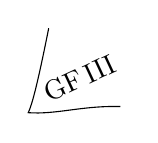
\begin{tikzpicture}[scale=.65]
\draw (.05,1.65) .. controls (-.10,.90) and (-.25,.20) .. (-.35,0) .. controls (.20,-.04) and (.70,.14) .. (1.45,.12);
\node[rotate=25] at (.65,.67) {GF\,\uline{III}};
\end{tikzpicture}}}

% slanted
\margin{\deleted{Ensembles} Parties \unsure{finies} de lieux \unsure{modérés|modérées}}

Je voudrais définir une autre axiomatique des \deleted{réseaux,}
\deleted{\unsure{l}}\unsure{la|a} structures de réseaux
sur un ens. $\mathcal L$ (\deleted{\unsure{d}}ens. des ``lieux'').

\textcircled{\scriptsize a}\quad $S_0\deleted{\unsure{(L)|L}}\subset P_2(L)$ l'ens des \uline{0-sphères}
\uline{plongées}, ou des \uline{paires} \deleted{\unsure{mod.}} (de
lieux) modérées. \inserted{si $\{a,b\}\in S_0$ ; on dit aussi que $a,b$ st \uline{disjoints} ou en position relative modérée.}

% slanted
\margin{Mais, on dit aussi que $a,b$ en position rel. modérée si $a=b$ \uline{ou} $\{a,b\}\in S_0$}

[En termes de l'axiomatique par les segments,
\unsure{cela|celà} signifie que \deleted{$a,b$ \unsure{sont} ou bien} \inserted{(à part $a,b$ \uline{distincts}},
\unsure{contenu} dans $\{a,b\}\in\deleted{\unsure{S_0}}P_2(\mathcal L)$, que
ou bien $\{a,b\}\cap\mathcal L_s\ne\varnothing$ ($a$ ou $b$ est un
nœud \unsure{sg$_r$|sg} du réseau) \uline{ou} \uline{bien} \deleted{$a,b$}
(si \deleted{\unsure{st|sont}} \inserted{$a,b$} réguliers) que $a,b$ \inserted{\unsure{doivt|doit}} \unsure{appartiennent|appartient} :
des lignes différentes, \unsure{soit|sont}, s'ils sont
dans une $\bar{=}$ ligne, que $\{a,b\}=\partial I$,
pour $I\in S$].

\deleted{\unsure{b)}} Une partie \uline{finie} \inserted{$T$} est dite \deleted{admissible} \inserted{``\uline{modérée}''}
si \deleted{$\forall\,a,b\in T$, \unsure{on a} $a,b$} $P_2(T)\subset S_0$
i.e. deux éléments quelc. de $T$ sont en
position relative modérée (\deleted{des} 2 à 2 ``disjoints'').

% paper watermark; faint outline impression
\rotatebox{90}{\textsc{\unsure{xtra Strong Ext}}}
